\documentclass{article}
\usepackage{amsmath}
\usepackage{mathtools}
\usepackage{gensymb}
\usepackage[a4paper,inner=1.5cm,outer=1.5cm,top=2cm,bottom=0.5cm]{geometry} 
\usepackage{xcolor}                    
\usepackage{tikz}                           
\usepackage{multicol}
\usepackage{hyperref}
\usepackage{pgfplots}
\usetikzlibrary{calc}
\usetikzlibrary{intersections}
\usetikzlibrary{intersections,calc,angles,quotes}
\usetikzlibrary{shapes,arrows,positioning,decorations.pathreplacing,calc}
\usetikzlibrary{calc,angles,positioning,intersections,quotes,decorations.markings}
\usepackage{tkz-euclide}
\usetikzlibrary{backgrounds}
\usetikzlibrary{calc,through}
\usetikzlibrary{angles}
\usetikzlibrary{fadings}
\usetikzlibrary{shapes.geometric}
\usetikzlibrary{shapes.symbols}
\usepackage{draftwatermark}
\usepackage{mathptmx}

\SetWatermarkText{\textcolor{black!10}{Mathema Shukur}}
\SetWatermarkFontSize{2 cm}
\usepackage[utf8]{inputenc}
\usepackage{fontspec}

\setmainfont{[Kalpurush.ttf]}
\newfontface{\en}{[Arial.ttf]} %%this is optional, if you want to use a secondary font. Any english font is supported
\newlength\Radius
\setlength\Radius{4cm}
\begin{document} 
	\Large
	একটি সরলরেখা দুইটি বৃত্তকে স্পর্শ করলে রেখাটিকে বৃত্ত দুইটির সাধারণ স্পর্শক (Common tangent)  বলে। সাধারণ স্পর্শক দুই প্রকারের।\\ 
	\\
(i) সরল সাধারণ স্পর্শক (Direct common tangent) \\
\\ 
(ii) তীর্যক সাধারণ স্পর্শক (Transverse common tangent )\\ 
\\ 
	দুইটি বৃত্তের সরল সাধারণ স্পর্শক $AB$ ও $AC$\\
	\\
	সাধারণ স্পর্শকের স্পর্শ বিন্দুদ্বয় বৃত্তের কেন্দ্রদ্বয়ের সংযোজক রেখার একই পার্শ্বে অবস্থিত হলে তাকে সরল সাধারণ স্পর্শক বলে \\ 
	\\
		\begin{tikzpicture}[transform shape,scale=0.5]
		\draw[thick,green] (0,0) circle (3);
		\fill[green] (0,0) circle (1 mm);
		\draw[thick,blue] (8,-1) circle (4);
		\fill[blue] (8,-1) circle (1 mm);
		\draw[cyan](-24,3)--(11,3);	
		\draw[cyan](-24,3)--(11.5,-6);
		\draw[red,dashed](0,0)--(8,-1);
		\node at (-24,2.5) {$\textcolor{red}{A}$};		
		\node at (11,2.5) {$\textcolor{red}{B}$};	
		\node at (11.5,-6.5) {$\textcolor{red}{C}$};	
	\end{tikzpicture}\\
	\\ 
পরস্পরচ্ছেদী নয় এমন  দুইটি বৃত্তের তীর্যক সাধারণ স্পর্শক $EF$ ও $GH$ \\
	\\
	 সাধারণ স্পর্শকের স্পর্শ বিন্দুদ্বয় কেন্দ্রদ্বয়ের সংযোজক রেখার বিপরীত পার্শ্বে অবস্থিত হলে তাকে তীর্যক সাধারণ স্পর্শক বলে। \\
		\begin{tikzpicture}[transform shape,scale=1]
		\draw[thick,green] (0,0) circle (3);
		\fill[green] (0,0) circle (0.5 mm);
		\draw[thick,blue] (8,-1) circle (4);
		\fill[blue] (8,-1) circle (0.5 mm);
		\draw[red](6,3)--(1.2,-3.4);	
		\draw[red](2,3)--(5.07,-4.38);
		\draw[red,dashed](0,0)--(8,-1);
		\node at (6,3.5) {$\textcolor{red}{E}$};		
		\node at (1.2,-4) {$\textcolor{red}{F}$};
		\node at (2,3.5) {$\textcolor{red}{G}$};		
		\node at (5,-5) {$\textcolor{red}{H}$};			
	\end{tikzpicture}\\
\\
$x^2+y^2=16$ এবং  $x^2+y^2+6x-8y=0$ বৃত্ত দুইটির সরল সাধারণ স্পর্শক দুইটির সমীকরণ নির্ণয় কর\\ 
\\
\begin{align*}
	x^2+y^2+6x-8y&=0\\
	\\
	x^2+y^2+2(3)x+2(-4)y&=0\\
	\boxed{\textcolor{blue}{x^2+y^2+2gx+2fy+c=0}}&\\
	g=3,\,\,f=-4,\,\,c&=0\\
\end{align*}
\begin{align*}
	(-g,-f) &=(-3,4)\\
	\\
	\sqrt{g^2+f^2-c}&=\sqrt{(3)^2+(-4)^2-0}\\
	&=\sqrt{9+16}\\
	&=\sqrt{25}\\
	&=5\\
\end{align*}
\\ 
$x^2+y^2+6x-8y=0$ বৃত্তের কেন্দ্র  $C_1(-3,4)$ ব্যাসার্ধ  $r_1=5$\\
\\
$x^2+y^2=4^2$ বৃত্তের কেন্দ্র $C_2(0,0)$ ব্যাসার্ধ $r_2=4$\\
\\ 
	\begin{tikzpicture}[transform shape,scale=0.5]
	\draw[thick,green] (-3,4) circle (5);
	\fill[green] (-3,4) circle (1 mm);
	\draw[thick,blue] (0,0) circle (4);
	\fill[blue] (0,0) circle (1 mm);
	\draw[red](12,-16)--(-9.4,3);	
		\draw[red](12,-16)--(0,9.35);
		\draw[cyan,dashed](-3,4)--(12,-16);	
	\draw[blue,dashed](0,0)--(3.6,1.71);
	\node at (2.5,0.8) {$\textcolor{blue}{4}$};		
		\draw[green,dashed](-3,4)--(1.51,6.13);	
	\node at (1,5.5) {$\textcolor{green}{5}$};	
	\node at (12.5,-16) {$\textcolor{red}{A}$};		
	\node at (-10,3) {$\textcolor{red}{B}$};	
		\node at (0,10) {$\textcolor{red}{C}$};	
		\node at (1.3,-0.3) {$\textcolor{blue}{C_2(0,0)}$};	
		\node at (-4,4.3) {$\textcolor{green}{C_1(-3,4)}$};
\end{tikzpicture}\\
\\
$C_1(-3,4)$ ও $C_2(0,0)$ কেন্দ্রদ্বয়ের সংযোগ রেখাংশ $A(x',y')$ বিন্দুতে  $r_1:r_2=5:4$ অনুপাতে বহিঃস্থ ভাবে বিভক্ত করে\\ 
\\ 
$x_1=-3,\,\,y_1=4,\,\,x_2=0,\,\,y_2=0$\\
\\
\begin{align*}
	x'&=\frac{r_1x_2-r_2x_1}{r_1-r_2}\\
	\\
	&=\frac{(5)(0)-(4)(-3)}{5-4}\\
	\\
	&=\frac{0+12}{1}\\
	\\
	&=12\\
\end{align*}
\\
\begin{align*}
	y'&=\frac{r_1y_2-r_2y_1}{r_1-r_2}\\
	\\
	&=\frac{(5)(0)-(4)(4)}{5-4}\\
	\\
	&=\frac{0-16}{1}\\
	\\
	&=-16\\
\end{align*}
\\
সরল সাধারণ স্পর্শক দুইটির ছেদবিন্দু $A(x',y')=A(12,-16)$\\
\\
$(12,-16)$ বিন্দুগামী সরলরেখার  সমীকরণ \\
\\ 
\begin{align*}
	(y-y')&=m(x-x')\\
	\boxed{\textcolor{blue}{x'=12,\,\,\,y'=-16}}&\\
	(y+16)&=m(x-12)\,\,\,[EQ01]\\
	\\
	y+16&=mx-12m\\
	\\
	mx-y-12m-16&=0\\
\end{align*}
\\
যদি $mx-y-12m-16=0$ সরলরেখাটি স্পর্শক হয় তবে \\
বৃত্তের কেন্দ্র $(0,0)$ থেকে $mx-y-12m-16=0$ রেখাটির  দূরত্ব  বৃত্তের ব্যাসার্ধ $(4)$ সমান হবে \\
\\  
\begin{align*}
	\frac{|m(0)-(0)-12m-16|}{\sqrt{m^2+1}}&=4\\
	\\
	\frac{|-12m-16|}{\sqrt{m^2+1}}&=4\\
	\\
	|3m+4|&=\sqrt{m^2+1}\\
	\\
	(3m+4)^2&=(\sqrt{m^2+1})^2\\
	\\
	9m^2+24m+16&=m^2+1\\
	\\
	8m^2+24m+15&=0\\
	\\
	m&=\frac{-24\pm\sqrt{(24)^2-4(8)(15)}}{2(8)}\\
	\\
	m&=\frac{-24\pm\sqrt{576-480}}{16}\\
	\\
	m&=\frac{-6\pm\sqrt{6}}{4}\\
\end{align*}
\\
\begin{align*}
	(y+16)&=m(x-12)\,\,[EQ01]\\
	\boxed{\textcolor{blue}{m=\frac{-6\pm\sqrt{6}}{4}}}&\\
	y+16&=\frac{-6\pm\sqrt{6}}{4}(x-12)\\
	\\
	4y+64&=(-6\pm\sqrt{6})(x-12)\\
	\\
	4y+64&=-6(x-12)\pm\sqrt{6}(x-12)\\
	\\
	4y+64+6(x-12)&=\pm\sqrt{6}(x-12)\\
	\\
	6x+4y-8&=\pm\sqrt{6}(x-12)\\
\end{align*}
\\
সরল সাধারণ স্পর্শকের সমীকরণ $6x+4y-8=\pm\sqrt{6}(x-12)$\\
\\
\textcolor{blue}{প্রশ্নঃ $x^2+y^2=9$ এবং  $x^2+y^2-16x+2y+49=0$ বৃত্তদ্বয়ের সাধারণ স্পর্শক নির্ণয় কর।}\\
\\ 
১ম ধাপঃ সরল সাধারণ স্পর্শক (Direct Common Tangent) \\
\\
২য় ধাপঃ তীর্যক সাধারণ স্পর্শক (Transverse Common Tangent) \\
\\ 
\begin{align*}
	x^2+y^2-16x+2y+49&=0\\
	\\
	x^2+y^2+2(-8)x+2(1)y+49&=0\\
	\\
	g&=-8\\
	\\
	f&=1\\
	\\
	c&=49\\
\end{align*}
\\
\begin{align*}
	(-g,-f)&=(8,-1)\\
	\\
	\sqrt{g^2+f^2-c}&=\sqrt{(-8)^2+(1)^2-49}\\
	\\
	&=\sqrt{64+1-49}\\
	\\
	&=\sqrt{65-49}\\
	\\
	&=\sqrt{16}\\
	\\
	&=4\\
\end{align*}
\\ 
 $x^2+y^2-16x+2y+49=0$ বৃত্তের কেন্দ্র  $C_1(8,-1)$ ও ব্যাসার্ধ  $r_1=4$\\
 \\
  $x^2+y^2=9$ বৃত্তের কেন্দ্র  $C_2(0,0)$ ও ব্যাসার্ধ  $r_2=3$\\
 \\ 
 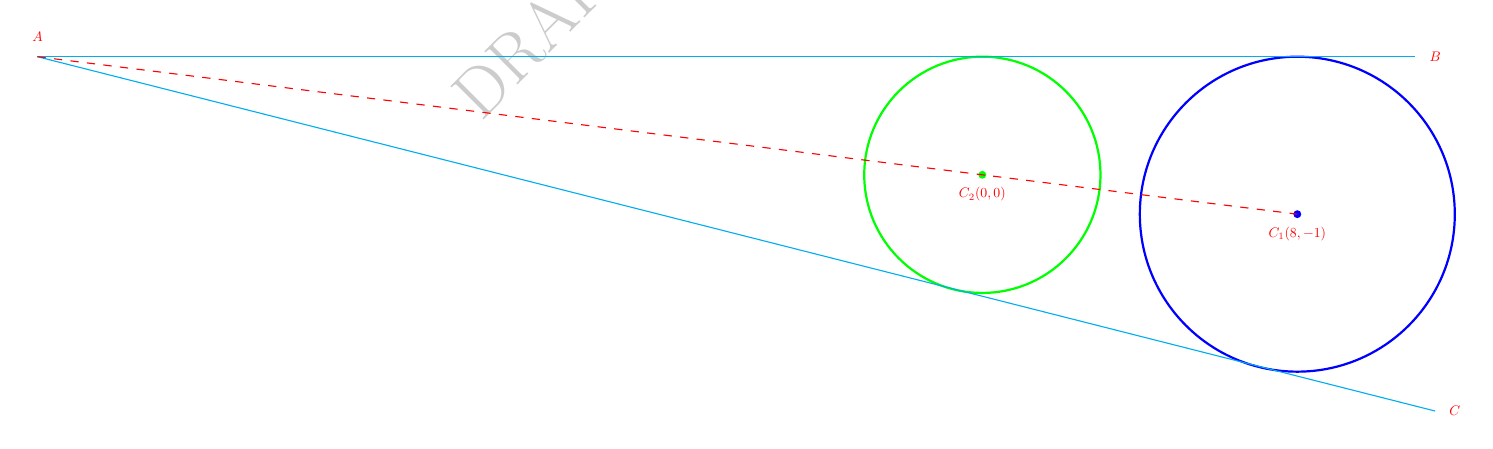
\begin{tikzpicture}[transform shape,scale=0.5]
 	\draw[thick,green] (0,0) circle (3);
 	\fill[green] (0,0) circle (1 mm);
 		\node at (0,-0.5) {$\textcolor{red}{C_2(0,0)}$};
 	\draw[thick,blue] (8,-1) circle (4);
 	\fill[blue] (8,-1) circle (1 mm);
 		\node at (8,-1.5) {$\textcolor{red}{C_1(8,-1)}$};
 	\draw[cyan](-24,3)--(11,3);	
 	\draw[cyan](-24,3)--(11.5,-6);
 	\draw[red,dashed](-24,3)--(8,-1);	
 	\node at (11.5,3) {$\textcolor{red}{B}$};		
 	\node at (12,-6) {$\textcolor{red}{C}$};	
  	\node at (-24,3.5) {$\textcolor{red}{A}$};			
 \end{tikzpicture}\\
 \\
 $C_1(8,-1)$ ও $C_2(0,0)$ কেন্দ্রদ্বয়ের সংযোগ রেখাংশ $A(x',y')$ বিন্দুতে  $r_1:r_2=4:3$ অনুপাতে বহিঃস্থ ভাবে বিভক্ত করে।  AB ও AC সরল সাধারণ স্পর্শক । \\ 
 \\ 
 বহির্বিভক্তির সেকশন ফর্মূলা প্রয়োগ করে A বিন্দুর স্থানাঙ্ক নির্ণয় করে পাই \\
\\ 
$x_1=8,\,\,y_1=-1,\,\,x_2=0,\,\,y_2=0,\,\,r_1=4,\,\,r_2=3$\\
\\
\begin{align*}
	x'&=\frac{r_1x_2-r_2x_1}{r_1-r_2}\\
	\\
	&=\frac{4(0)-3(8)}{4-3}\\
	\\
	&=\frac{0-24}{1}\\
	\\
	&=-24\\
\end{align*}
\\
\begin{align*}
	y'&=\frac{r_1y_2-r_2y_1}{r_1-r_2}\\
	\\
	&=\frac{4(0)-3(-1)}{4-3}\\
	\\
	&=\frac{3}{1}\\
	\\
	&=3\\
\end{align*}
\\
সরল সাধারণ স্পর্শক দুইটির ছেদবিন্দু $A(x',y')=A(-24,3)$\\
\\
$(-24,3)$ বিন্দুগামী সরলরেখার  সমীকরণ \\
\\ 
\begin{align*}
	(y-y')&=m(x-x')\\
	\\
	y-3&=m(x+24)\,\,\,[EQ01]\\
	\\
	y-3&=mx+24m\\
	\\
	mx-y+24m+3&=0\\
\end{align*}
\\
যদি $mx-y+24m+3=0$ সরলরেখাটি স্পর্শক হয় তবে \\
বৃত্তের কেন্দ্র $(0,0)$ থেকে $mx-y+24m+3=0$ রেখাটির  দূরত্ব  বৃত্তের ব্যাসার্ধ $(3)$ সমান হবে \\
\\  
\begin{align*}
	\frac{|m(0)-(0)+24m+3|}{\sqrt{m^2+1}}&=3\\
	\\
	\frac{|24m+3|}{\sqrt{m^2+1}}&=3\\
	\\
	|8m+1|&=\sqrt{m^2+1}\\
	\\
	(8m+1)^2&=(\sqrt{m^2+1})^2\\
	\\
	64m^2+16m+1&=m^2+1\\
	\\
	63m^2+16m&=0\\
	\\
	m(63m+16)&=0\\
	\\
	m&=0,-\frac{16}{63}\\
\end{align*}
\\
\begin{align*}
	(y-3)&=m(x+24)\,\,\,[EQ01]\\
	\boxed{\textcolor{blue}{m=0}}&\\
	(y-3)&=(0)(x+24)\\
	\\
	y-3&=0\\
\end{align*}
\\ 
AB সরল সাধারণ স্পর্শকের সমীকরণ $y-3=0$\\
\\
\begin{align*}
		y-3&=m(x+24)\,\,\,[EQ01]\\
	\boxed{\textcolor{blue}{m=-\frac{16}{63}}}&\\
	y-3&=-\frac{16}{63}(x+24)\\
\\
	63y+189&=-16x+384\\
	\\
16x+63y+195&=0\\
\end{align*}
\\ 
AC সরল সাধারণ স্পর্শকের সমীকরণ $16x+63y+195=0$\\
\\
	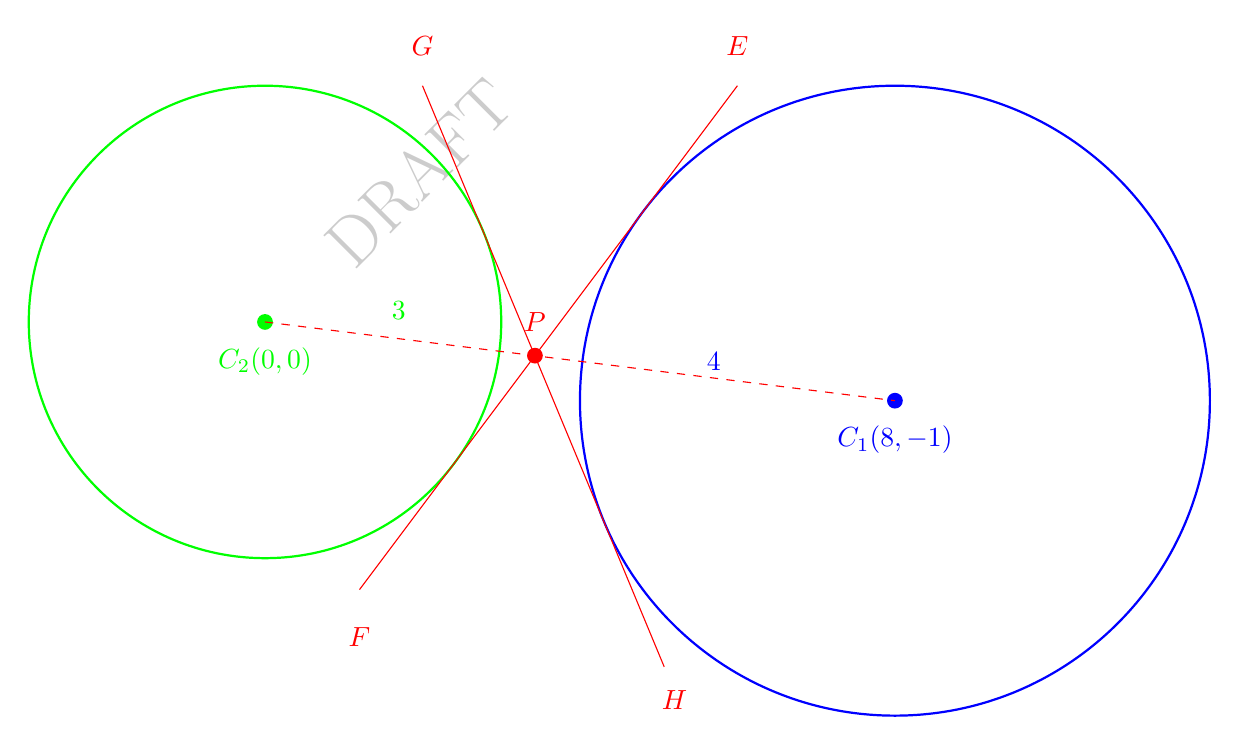
\begin{tikzpicture}[transform shape,scale=1]
	\draw[thick,green] (0,0) circle (3);
	\fill[green] (0,0) circle (1 mm);
	\draw[thick,blue] (8,-1) circle (4);
	\fill[blue] (8,-1) circle (1 mm);
	\draw[red](6,3)--(1.2,-3.4);
	\node at (6,3.5) {$\textcolor{red}{E}$};
	\node at (1.2,-4) {$\textcolor{red}{F}$};	
	\draw[red](2,3)--(5.07,-4.38);
		\node at (2,3.5) {$\textcolor{red}{G}$};
	\node at (5.2,-4.8) {$\textcolor{red}{H}$};	
		\draw[red,dashed](0,0)--(8,-1);
	\fill[red] (3.428,-0.428) circle (1 mm);
	\node at (3.428,0) {$\textcolor{red}{P}$};		
	\node at (0,-0.5) {$\textcolor{green}{C_2(0,0)}$};	
\node at (8,-1.5) {$\textcolor{blue}{C_1(8,-1)}$};			
\node at (5.70,-0.5) {$\textcolor{blue}{4}$};	
\node at (1.70,0.15) {$\textcolor{green}{3}$};			
\end{tikzpicture}
\\ 
 $C_1(8,-1)$ ও $C_2(0,0)$ কেন্দ্রদ্বয়ের সংযোগ রেখাংশ $P(x'',y'')$ বিন্দুতে  $r_1:r_2=4:3$ অনুপাতে অন্তঃস্থ ভাবে বিভক্ত করে। তীর্যক সাধারণ স্পর্শক দুইটি হলো EF ও  GH \\ 
\\ 
অন্তর্বিভক্তির সেকশন ফর্মুলা প্রয়োগ করে P বিন্দুর স্থানাঙ্ক নির্ণয় করে পাই  \\
\\ 
$x_1=8,\,\,y_1=-1,\,\,x_2=0,\,\,y_2=0,\,\,r_1=4,\,\,r_2=3$\\
\\
\begin{align*}
	x''&=\frac{r_1x_2+r_2x_1}{r_1+r_2}\\
	\\
	&=\frac{4(0)+3(8)}{4+3}\\
	\\
	&=\frac{24}{7}\\
\end{align*}
\\
\begin{align*}
	y''&=\frac{r_1y_2+r_2y_1}{r_1+r_2}\\
	\\
	&=\frac{4(0)+3(-1)}{4+3}\\
	\\
	&=-\frac{3}{7}\\
\end{align*}
\\
তীর্যক সাধারণ স্পর্শক দুইটির ছেদবিন্দু $P(x'',y'')=P\left(\frac{24}{7},-\frac{3}{7}\right)$\\
\\
$\left(\frac{24}{7},-\frac{3}{7}\right)$ বিন্দুগামী সরলরেখার  সমীকরণ \\
\\ 
\begin{align*}
	(y-y'')&=m(x-x'')\\
	\\
	(y+\frac{3}{7})&=m(x-\frac{24}{7})\\
	\\
	7y+3&=7mx-24m\\
	\\
	7mx-7y-24m+3&=0\\
\end{align*}
\\
যদি $7mx-7y-24m+3=0$ সরলরেখাটি স্পর্শক হয় তবে \\
বৃত্তের কেন্দ্র $(0,0)$ থেকে $7mx-7y-24m+3=0$ রেখাটির  দূরত্ব  বৃত্তের ব্যাসার্ধ $(3)$ সমান হবে \\
\\  
\begin{align*}
	\frac{|7m(0)-7(0)-24m-3|}{\sqrt{(7m)^2+(-7)^2}}&=3\\
	\\
	\frac{|-24m-3|}{7\sqrt{m^2+1}}&=3\\
	\\
	|8m+1|&=7\sqrt{m^2+1}\\
	\\
	(8m+1)^2&=(7\sqrt{m^2+1}^2)\\
	\\
	64m^2+16m+1&=49(m^2+1)\\
	\\
	64m^2+16m+1&=49m^2+49\\
	\\
	64m^2-49m^2+16m-48&=0\\
	\\
	15m^2+16m-48&=0\\
	\\
	(3m-4)(5m+12)&=0\\
	\\
	m&=\frac{4}{3},-\frac{12}{5}\\
\end{align*}
\\
\begin{align*}
	\left(y+\frac{3}{7}\right)&=m\left(x-\frac{24}{7}\right)\\
	\boxed{\textcolor{blue}{m=\frac{4}{3}}}&\\
	\left(y+\frac{3}{7}\right)&=\frac{4}{3}\left(x-\frac{24}{7}\right)\\
	\\
	21y+9&=28x-96\\
	\\
	28x-21y-105&=0\\
	\\
	4x-3y-15&=0\\
\end{align*}
\\
EF তীর্যক সাধারণ স্পর্শকের সমীকরণ  $4x-3y-15=0$\\
\\ 
\begin{align*}
	\left(y+\frac{3}{7}\right)&=m\left(x-\frac{24}{7}\right)\\
	\boxed{\textcolor{blue}{m=-\frac{12}{5}}}&\\
	\left(y+\frac{3}{7}\right)&=-\frac{12}{5}\left(x-\frac{24}{7}\right)\\
	\\
	35y+15&=-84x+288\\
	\\
	84x+35y-273&=0\\
	\\
	12x+5y-39&=0\\
\end{align*}
\\
GH তীর্যক সাধারণ স্পর্শকের সমীকরণ  $12x+5y-39=0$\\
\\
	দেখাও যে, $x^2+y^2-2x+4y-31=0$ এবং $x^2+y^2+4x-4y+7=0$ বৃত্তদ্বয় পরস্পরকে অন্তঃস্থ ভাবে স্পর্শ করে। সাধারণ স্পর্শক ও স্পর্শ বিন্দুর স্থানাঙ্ক নির্ণয় কর \\ 
\\
\begin{tikzpicture}[transform shape,scale=1]
	\draw[thick,green] (1,-2) circle (6);
	\fill[green] (1,-2) circle (0.5 mm);
	\draw[thick,blue] (-2,2) circle (1);
	\fill[blue] (-2,2) circle (0.5 mm);
	\draw[red](-5,1)--(-1,4);	
	\fill[red] (-3,0) circle (1 mm);
	\fill[red] (-1,2) circle (1 mm);
	\node at (-3.5,0) {$\textcolor{red}{A}$};		
	\node at (-1,2.5) {$\textcolor{red}{B}$};		
\end{tikzpicture}\\
\\ 
\begin{align*}
	x^2+y^2-2x+4y-31&=0\\
	\\
	x^2+y^2+2(-1)x+2(2)y+(-31)&=0\\
	\\
	g&=-1\\
	\\
	f&=2\\
	\\
	c&=-31\\
\end{align*}
\\
\begin{align*}
	(-g,-f)&=(1,-2)\\
	\\
	\sqrt{g^2+f^2-c}&=\sqrt{(-1)^2+(2)^2+31}\\
	\\
	\sqrt{g^2+f^2-c}&=\sqrt{1+4+31}\\
	\\
	&=\sqrt{36}\\
	\\
	&=6\\
\end{align*}
\\
\begin{align*}
	x^2+y^2+4x-4y+7&=0\\
	\\
	x^2+y^2+2(2)x+2(-2)y+7&=0\\
	\\
	g&=2\\
	\\
	f&=-2\\
	\\
	c&=7\\
\end{align*}
\\
\begin{align*}
	(-g,-f)&=(-2,2)\\
	\\
	\sqrt{g^2+f^2-c}&=\sqrt{(2)^2+(-2)^2-7}\\
	\\
	&=\sqrt{4+4-7}\\
	\\
	&=\sqrt{1}\\
	\\
	&=1\\
\end{align*}
\\
\begin{align*}
	(x^2+y^2-2x+4y-31)-(x^2+y^2+4x-4y+7)&=0\\
	\\
	x^2+y^2-2x+4y-31-x^2-y^2-4x+4y-7&=0\\
	\\
	-6x+8y-38&=0\\
	\\
	3x-4y+19&=0\\
\end{align*}
\\
\begin{align*}
	\frac{y-y_1}{y_1-y_2}&=\frac{x-x_1}{x_1-x_2}\\
	\\
	\frac{y+2}{-2-2}&=\frac{x-1}{1+2}\\
	\\
	\frac{y+2}{-4}&=\frac{x-1}{3}\\
	\\
	3(y+2)&=-4(x-1)\\
	\\
	3y+6&=-4x+4\\
	\\
	4x+3y+2&=0\\
\end{align*}
\end{document}